


% (20\% of Report Length)

% a. Showcase the output at various intermediate stages of the project pipeline

% b. Use proper data visualizing techniques to present the output

% c. Figures and tables must be accompanied by an explanation

\chapter{RESULTS AND ANALYSIS}

\section{Model Training Analysis}
\vspace{10pt} % Adjust the value as needed
SABDA-NER is a Nepali Named Entity Recognition (NER) model. It was trained on a dataset consisting of 16,000 training examples and validated with 4,700 instances. The dataset was curated from various sources of Nepali Corpus data, supplemented by a manually created dataset of 1,700 examples for testing purposes.\\
\\
Prior to training, we merged datasets from Everest and WikiANN, preparing them for training on the pre-trained multilingual cased model. While the multilingual model is designed for various languages, it struggles with Nepali named entities. However, it effectively recognizes Devanagari script, leading us to choose this model for training.\\
\\
The training process, conducted on a T4 GPU with approximately 15GB of available RAM in Google Colab, took around 1 hour. The visualizations of the training process and corresponding F1 scores are depicted in the charts and table below.


 
Given the contextual nature of the model, predictions may be more accurate and incorrect for words out of context. As the data primarily comprises official documentation sentences, which are more contextual than casual conversations, this contextual limitation exists. \\
\\
Looking ahead, our future work involves testing the model on a larger dataset. The current evaluation is based on a relatively small set of sentences, and exploring its performance on a larger scale with out of contextual data is essential. Our initial findings indicate room for improvement, especially in handling out-of-context words.
\newpage
\subsection{Score Result after Training Model}

 
\begin{table}[H]
  
    \centering
    
    \begin{tabular}{|c|c|c|}
        % \hline
        % Column 1 & Column 2 & Column 3 \\
        % \hline
        % Row 1, Cell 1 & Row 1, Cell 2 & Row 1, Cell 3 \\
        % Row 2, Cell 1 & Row 2, Cell 2 & Row 2, Cell 3 \\
        % \hline
    \end{tabular}
    
    
\end{table}

\begin{figure}[H]
\centering
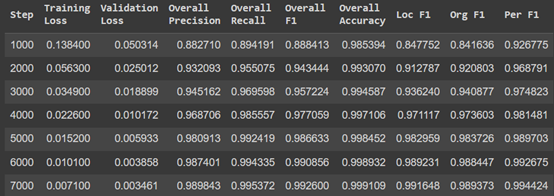
\includegraphics [scale=1]{img/result & analysis/image9.png}
\caption{ Score Result after Training Model}
\label{tab:  Score Result after Training Model}
% \caption[ Model Training Analysis]{Model Training Analysis}
% \label{fig:DisplaCy.png}

\end{figure}
 
 
\textbf{eval vs overall\_precision chart}

The chart above illustrates the ongoing improvement in precision as training progresses, with higher evaluation numbers contributing to the enhancement.


\begin{figure}[H]
\centering
\includegraphics [scale=0.45]{img/result & analysis/eval vs overall\_precision chart.png}
 \caption[ eval vs overall\_precision chart]{eval vs overall\_precision chart}
% \label{fig:DisplaCy.png}

\end{figure}

\newpage
\textbf{train vs training loss chart}

The "Train vs Training Loss" chart illustrates a decline in loss as the number of training datasets increases. Initially starting with maximum loss, the trend indicates a convergence towards zero, aligning with the expectation that training loss should be minimized.

\vspace{20pt}

 \begin{figure}[H]
\centering
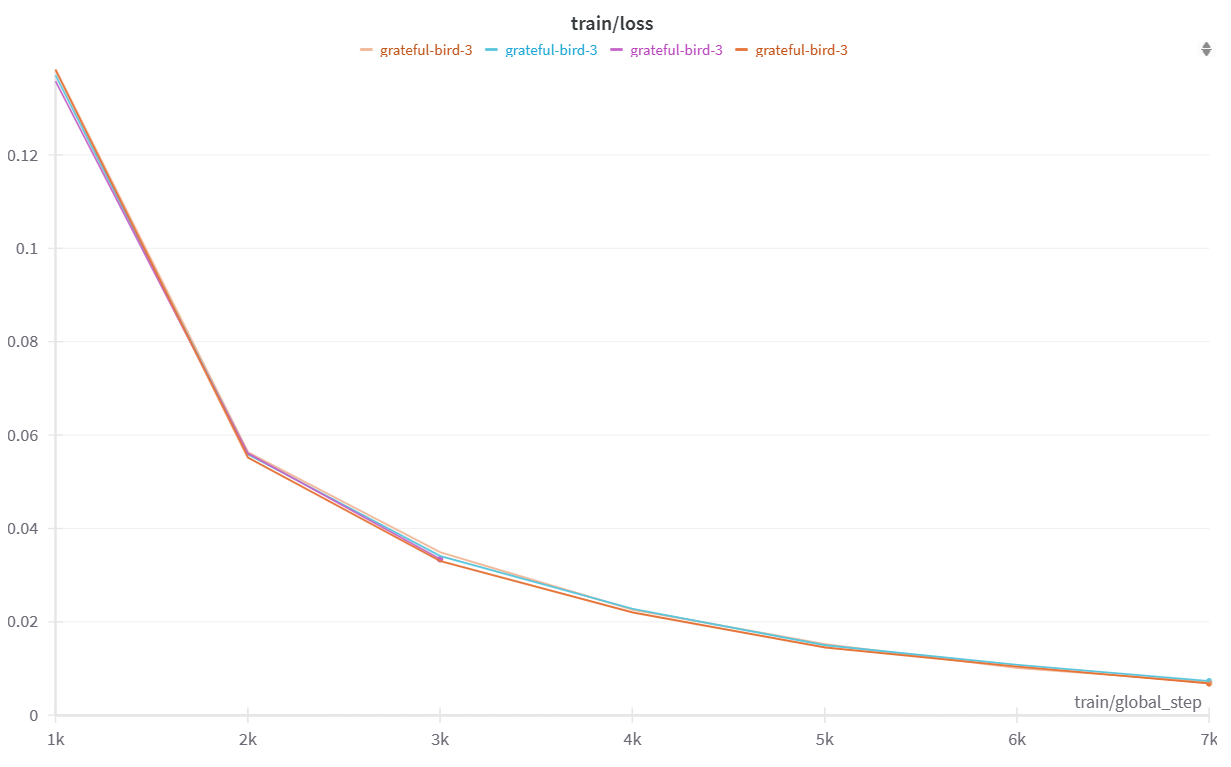
\includegraphics [scale=0.55]{img/result & analysis/train vs training loss chart.png}
 \caption[ train vs training loss chart]{train vs training loss chart}
% \label{fig:DisplaCy.png}

\end{figure}
 

\newpage

\textbf{Train vs epoch}
\begin{figure}[H]
\centering
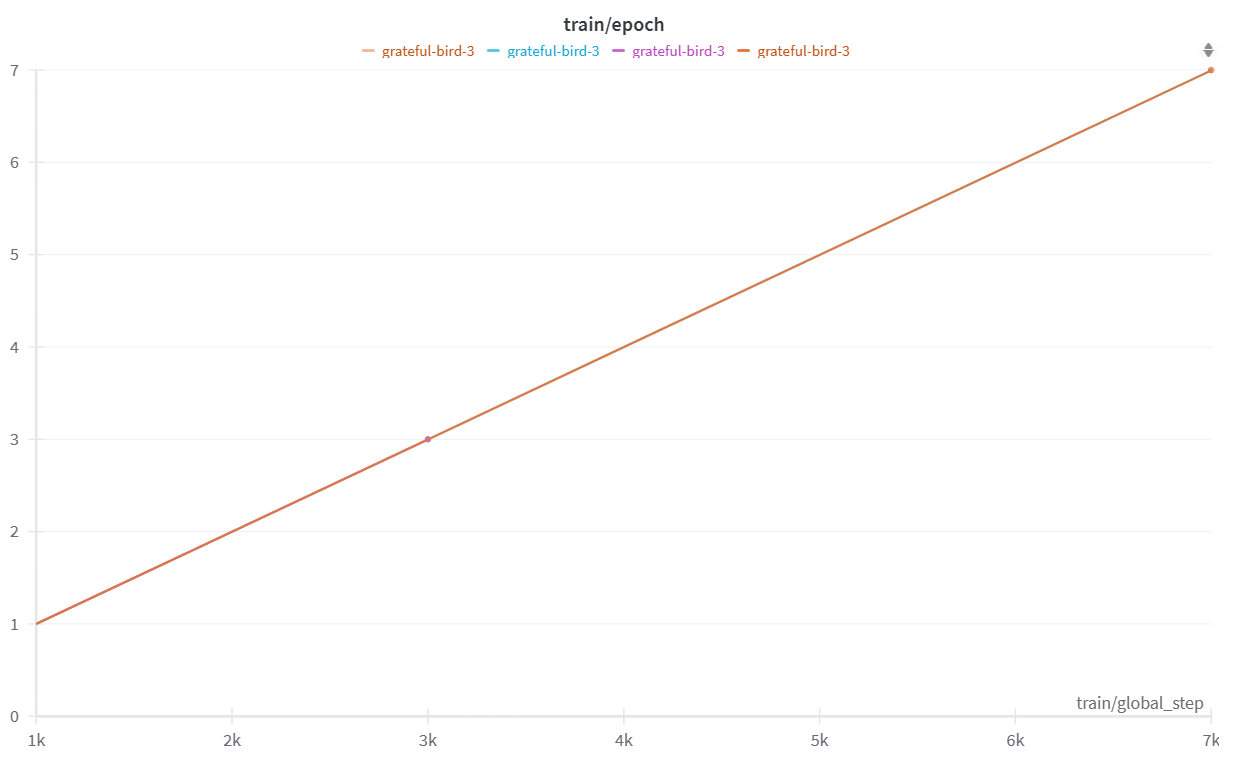
\includegraphics [scale=0.45]{img/result & analysis/Train vs epoch.png}
 \caption[Train vs epoch]{Train vs epoch}
% \label{fig:DisplaCy.png}

\end{figure}
 
 
"Train vs Epoch" depicts the training progress over epochs. Given a total of 7,000 evaluations to train and a chosen epoch of 7, the chart indicates a linear pattern. Each epoch involves training 1,000 evaluations, completing the entire set by the 7th epoch.

\textbf{Evaluation vs Loss}

"Evaluation vs Loss" illustrates the relationship between the evaluation process and the loss incurred during training. As the number of evaluations increases over the selected epochs, the chart reflects the corresponding decrease in the loss. This downward trend signifies that the model is progressively improving its predictive performance, achieving a lower loss value as it undergoes more training evaluations. The linear pattern suggests a consistent reduction in loss, demonstrating the effectiveness of the training process. By the 7th epoch, the model has undergone sufficient training to address the entire set of 7,000 evaluations, showcasing a comprehensive learning trajectory.

\begin{figure}[H]
\centering
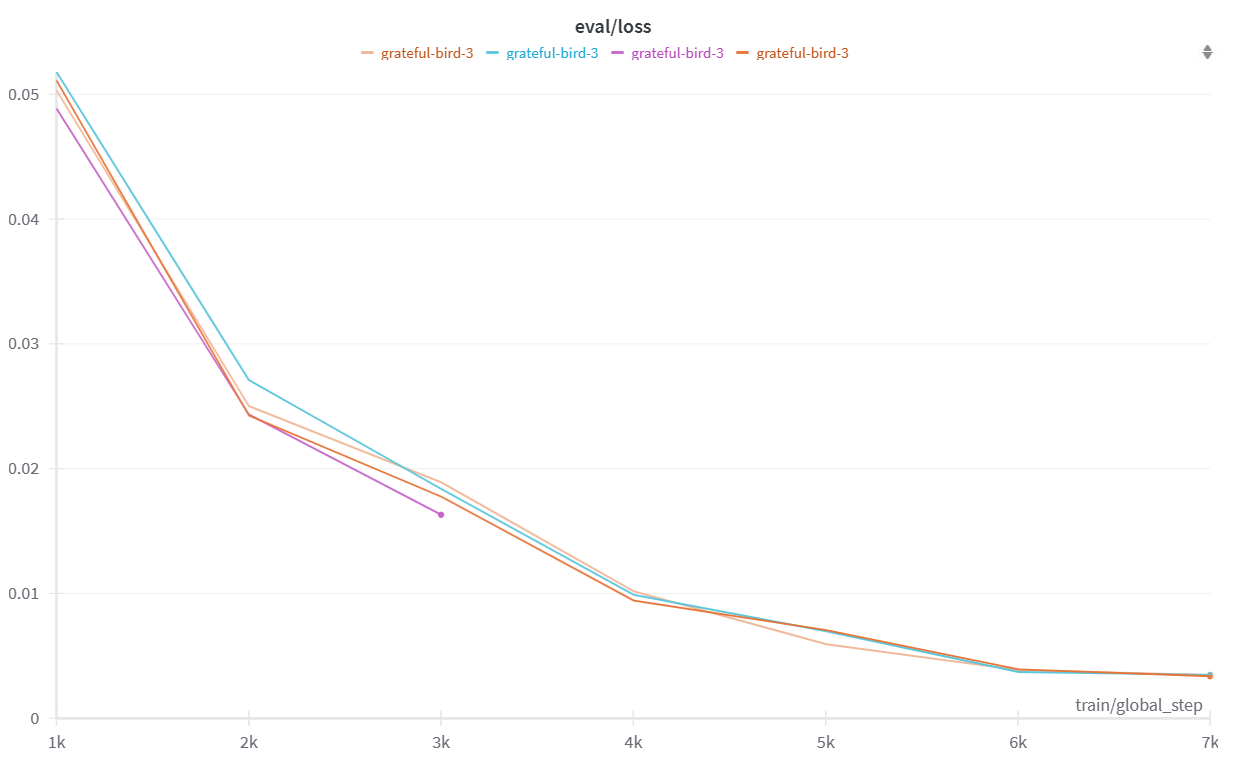
\includegraphics [scale=0.55]{img/result & analysis/Eval vs Loss.png}
 \caption[Eval vs Loss]{Eval vs Loss}
% \label{fig:DisplaCy.png}

\end{figure}

 

\textbf{eval vs overall\_f1}

\begin{figure}[H]
\centering
\includegraphics [scale=0.4]{img/result & analysis/eval vs overall\_f1.png}
 \caption[eval vs overall\_f1]{eval vs overall\_f1}
% \label{fig:DisplaCy.png}

\end{figure}

 
The "Evaluation vs Overall F1" chart visually represents the relationship between the evaluation process and the overall F1 score during model training. F1 score is a metric that balances precision and recall, providing a holistic measure of a model's performance.\\
\\
As the number of evaluations increases over epochs, the chart showcases the corresponding behavior of the overall F1 score. A rising trend in the overall F1 score indicates an improvement in the model's ability to correctly classify and identify entities. The chart offers insights into how well the model is performing across the entire dataset, with higher F1 scores signifying better overall predictive accuracy. Analyzing the fluctuations and trends in the chart allows for a nuanced understanding of the model's learning dynamics and its effectiveness in handling different types of entities in the given context.



\section{Resource Utilization Analysis}
\vspace{10pt}
\textbf{Power of GPU usage over time}

Figure 6 shows the utilization of GPU power over time. The chart indicates that the GPU is predominantly employed to its full capacity, with occasional declines, possibly attributed to network issues or optimization. Despite minor fluctuations of around ±10 in the data readings, the chart consistently reflects the efficiency of the network, as indicated by WandB.\\
\\
All the above charts were develop with the help of W\&B machine learning visualization library, with the help of it we can visualize our training model live through its website, after providing some data about the model training to the library.

\begin{figure}[H]
\centering
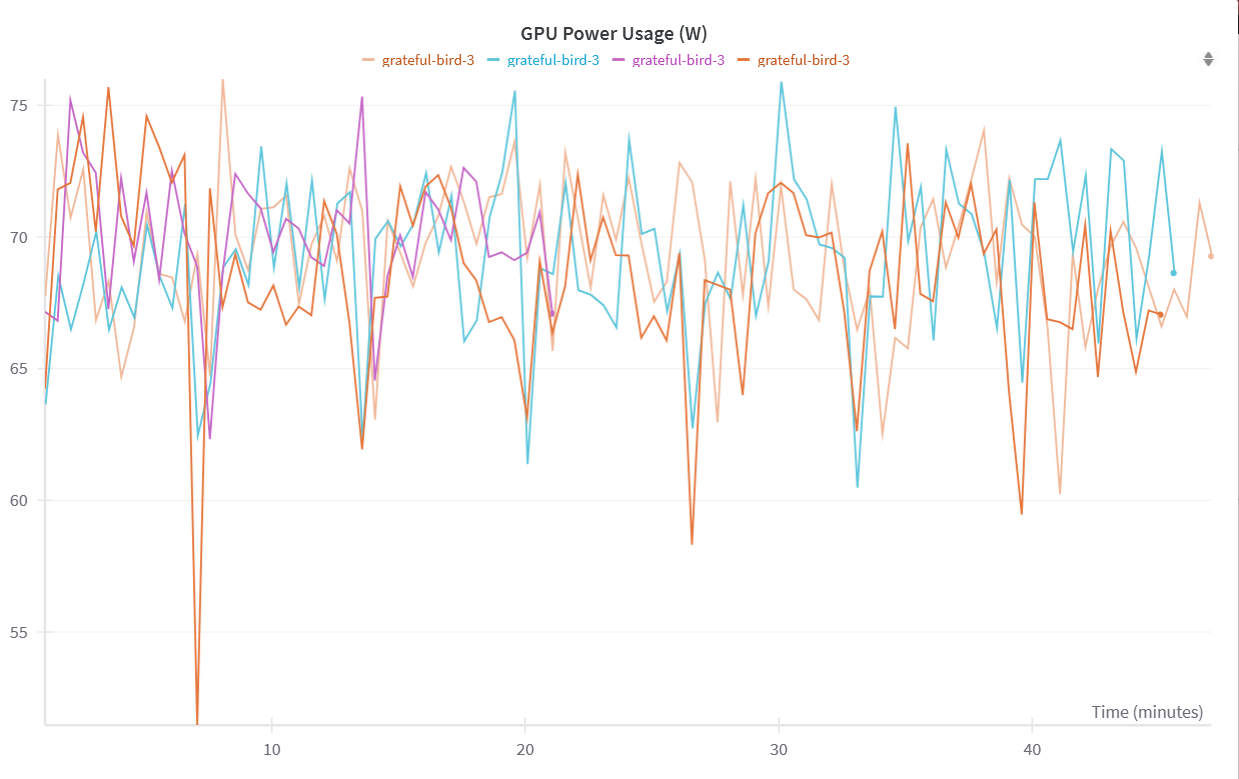
\includegraphics [scale=0.55]{img/result & analysis/Power of GPU usage over time.png}
 \caption[Power of GPU usage over times]{Power of GPU usage over time}
% \label{fig:DisplaCy.png}

\end{figure}

 



\section{Test Result}
\vspace{10pt}

The test of sentence that is manually imported for variable sentence as,
sentence = 
\begin{figure}[H]
\centering
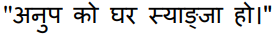
\includegraphics [scale=1.5]{img/result & analysis/anupKOghar.png}
 %\caption[Power of GPU usage over times]{Power of GPU usage over time}
% \label{fig:DisplaCy.png}

\end{figure}

 
This test sentence’s output is shown in other figure with entity list label and the respective scores. As we put the numbering to the label which as:

label\_names = ['O', 'B-PER', 'I-PER', 'B-ORG', 'I-ORG', 'B-LOC', 'I-LOC']

In the array the label start with:\\
0 -\> Other\\
1 -\> B-PER\\
2 -\> I-PER Figure\\
3 -\> B-ORG\\
4 -\> I-ORG\\
5 -\> B-LOC\\
6 -\> I-LOC\\

\begin{figure}[H]
\centering
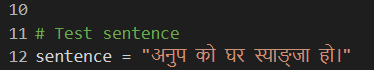
\includegraphics [scale=1.5]{img/result & analysis/Test sentence.png}
 \caption[Test sentence]{Test sentence}
% \label{fig:DisplaCy.png}

\end{figure}

 
The results shown by the model is pretty good with high score , i.e above 90 in each of the entity. Which shows the models result is found to be excellent.

\begin{figure}[H]
\centering
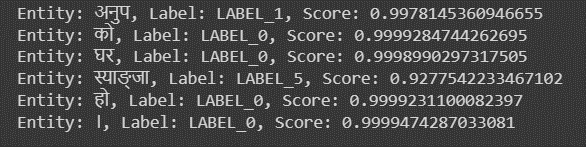
\includegraphics [scale=0.95]{img/result & analysis/Test results.png}
 \caption[Test results]{Test results}
% \label{fig:DisplaCy.png}

\end{figure}

 
\newpage
\section{Result Format}
\vspace{10pt}

We Anticipating the delivery of the project output through a website interface, users will be empowered to input sentences in the Nepali language. Subsequently, our model will diligently identify and extract Named Entities from the supplied text, enhancing the user experience and providing valuable insights.

\begin{figure}[H]
\centering
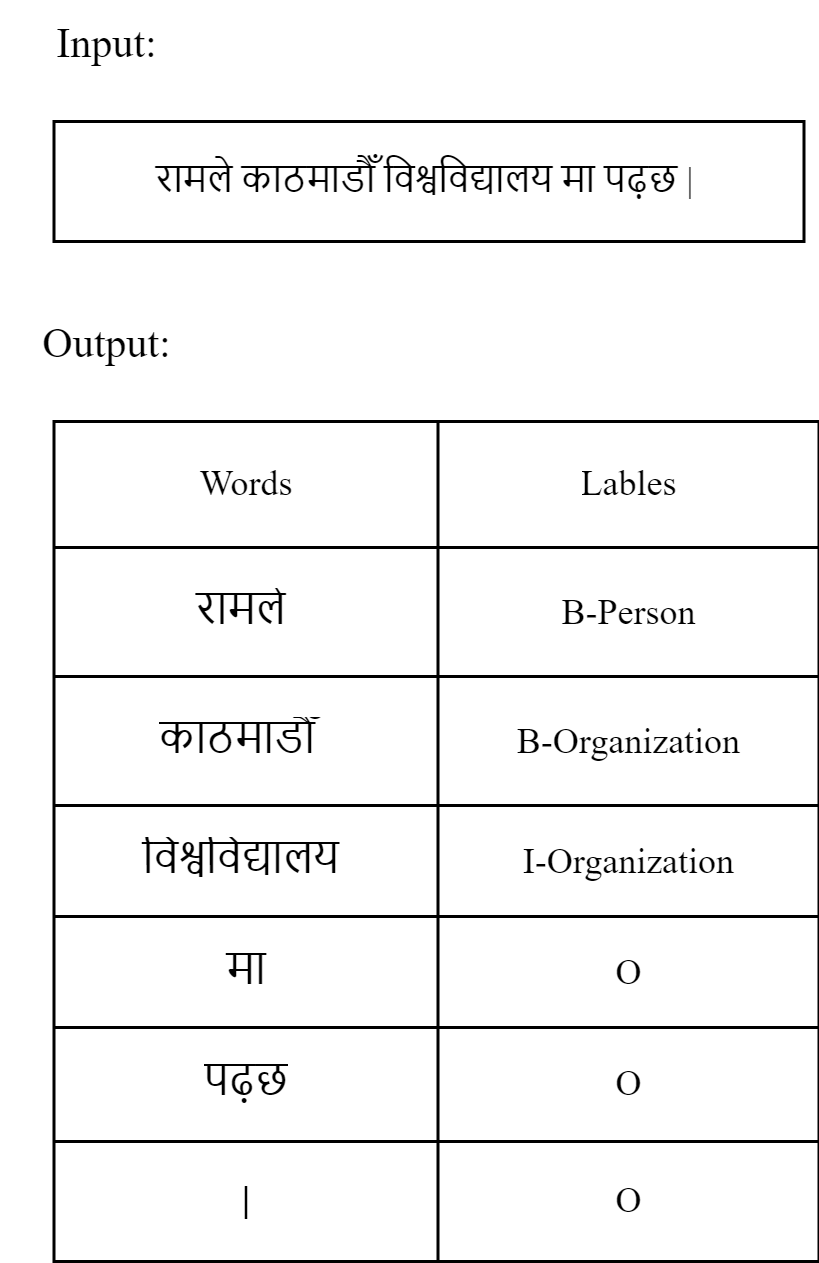
\includegraphics [scale=1.6]{img/result & analysis/_Input_output.png}
 \caption[Result Format]{Result Format}
% \label{fig:DisplaCy.png}

\end{figure}



\newpage
\section{UI}
\vspace{20pt}



\begin{figure}[H]
\centering
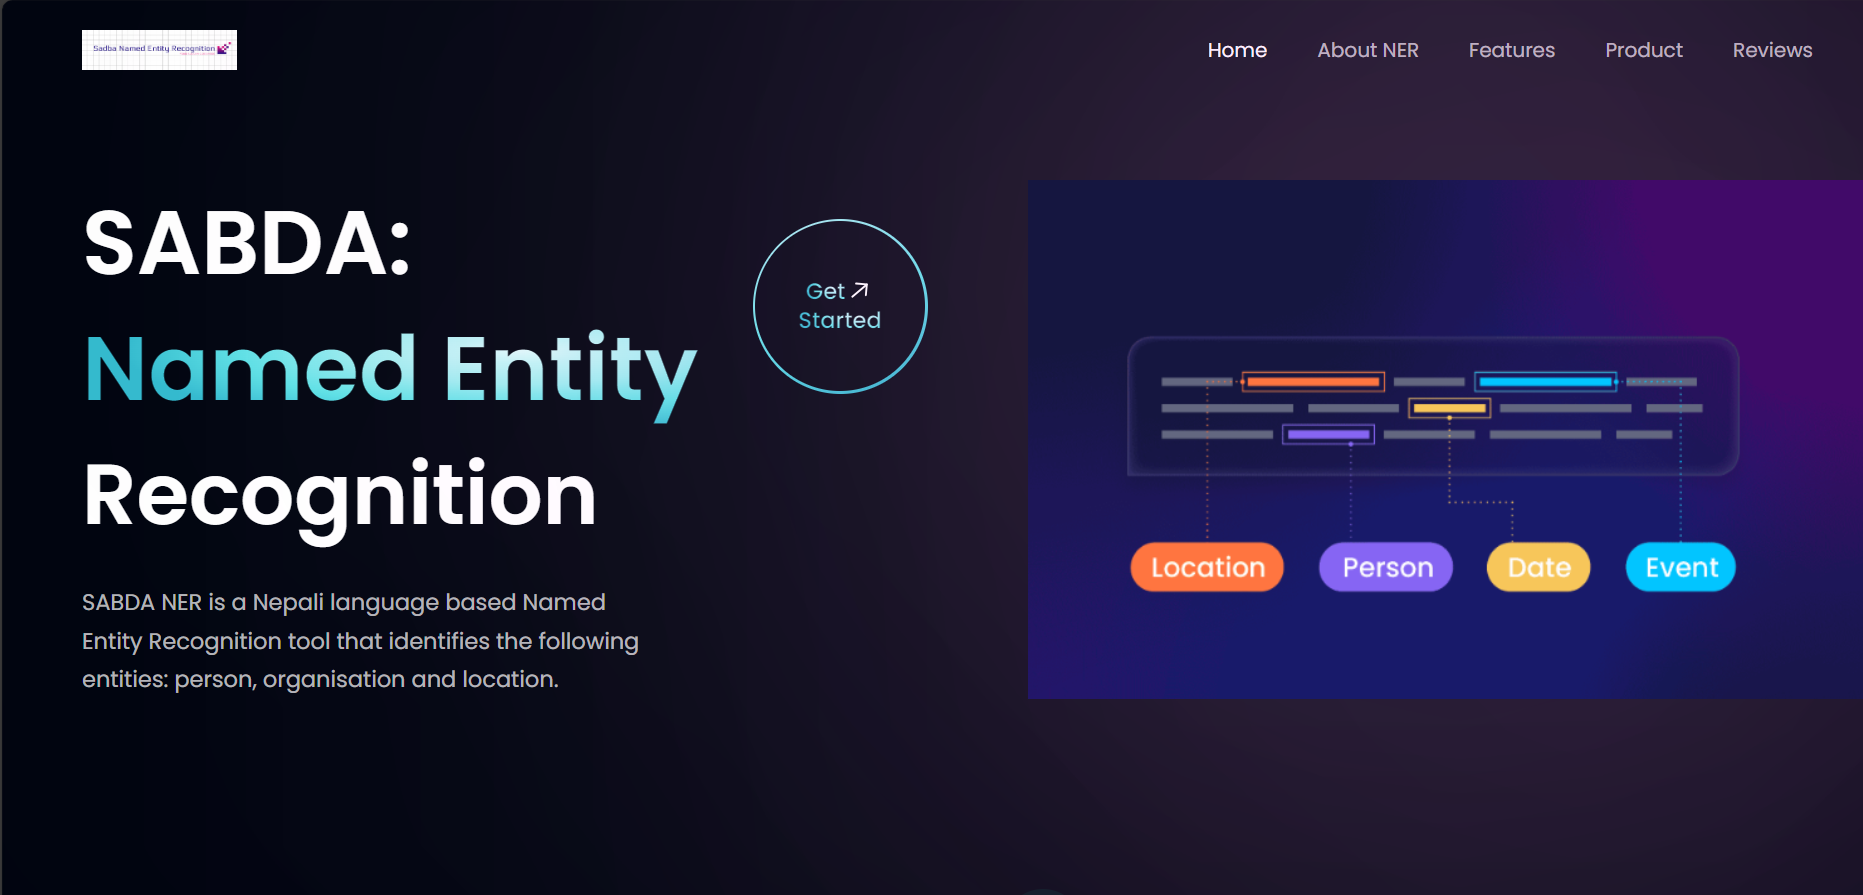
\includegraphics [scale=0.37]{img/UI/1home.png}
 \caption[Home Page]{Home Page}
% \label{fig:DisplaCy.png}

\end{figure}

\vspace{30pt}

\begin{figure} [H]
    \centering
    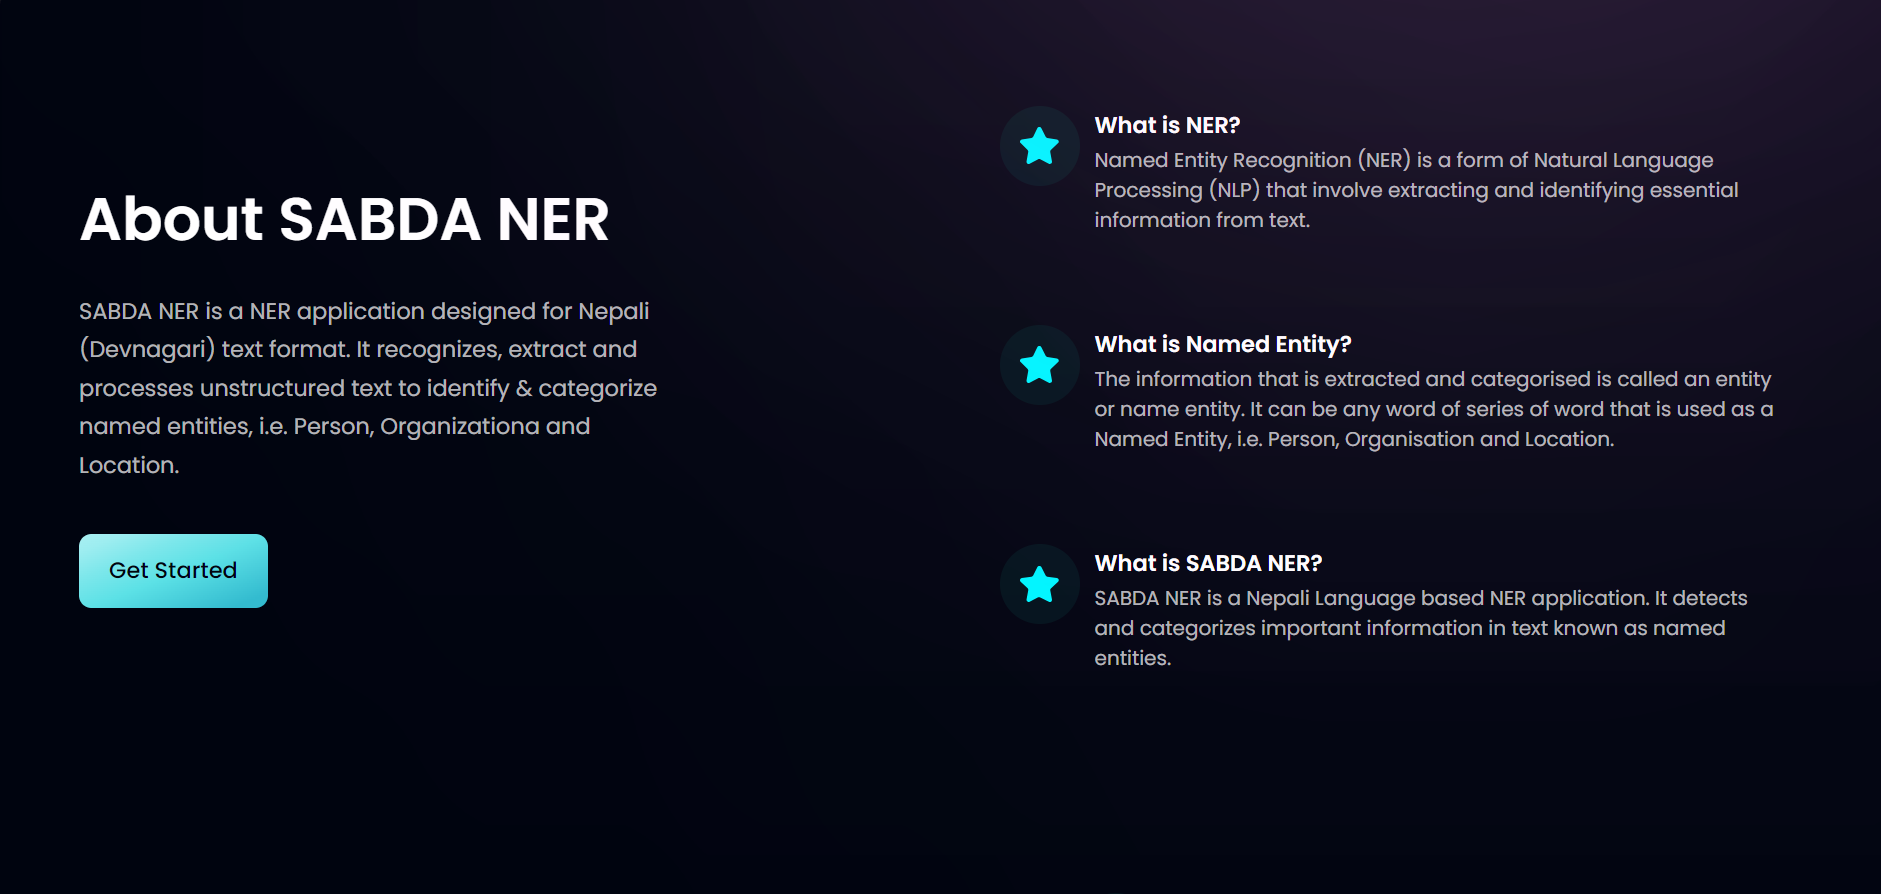
\includegraphics [scale=0.37]{img/UI/2about.PNG}
    \caption [About NER]{About NER}
    %\label{fig:enter-label}
\end{figure} 

\vspace{30pt}

\begin{figure}[H]
\centering
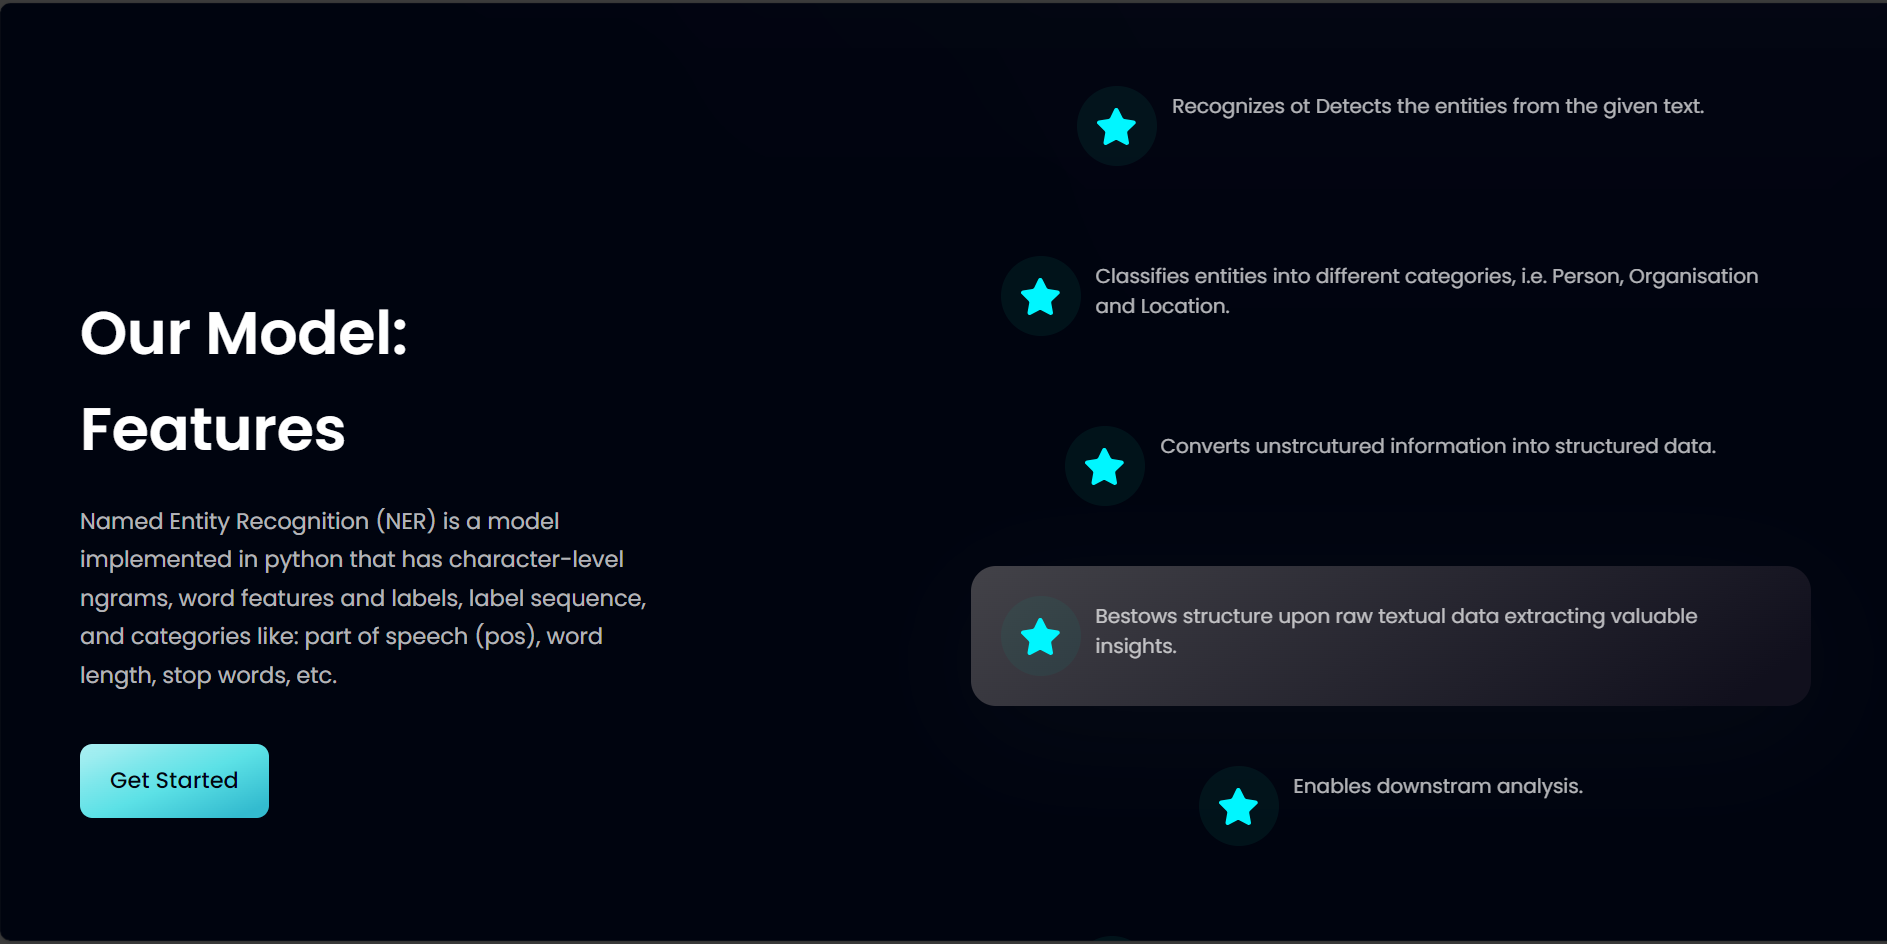
\includegraphics [scale=0.37]{img/UI/3feature.png}
 \caption[Features Page]{Features Page}
% \label{fig:DisplaCy.png}
\end{figure}

\vspace{30pt}
 
\begin{figure}[H]
\centering
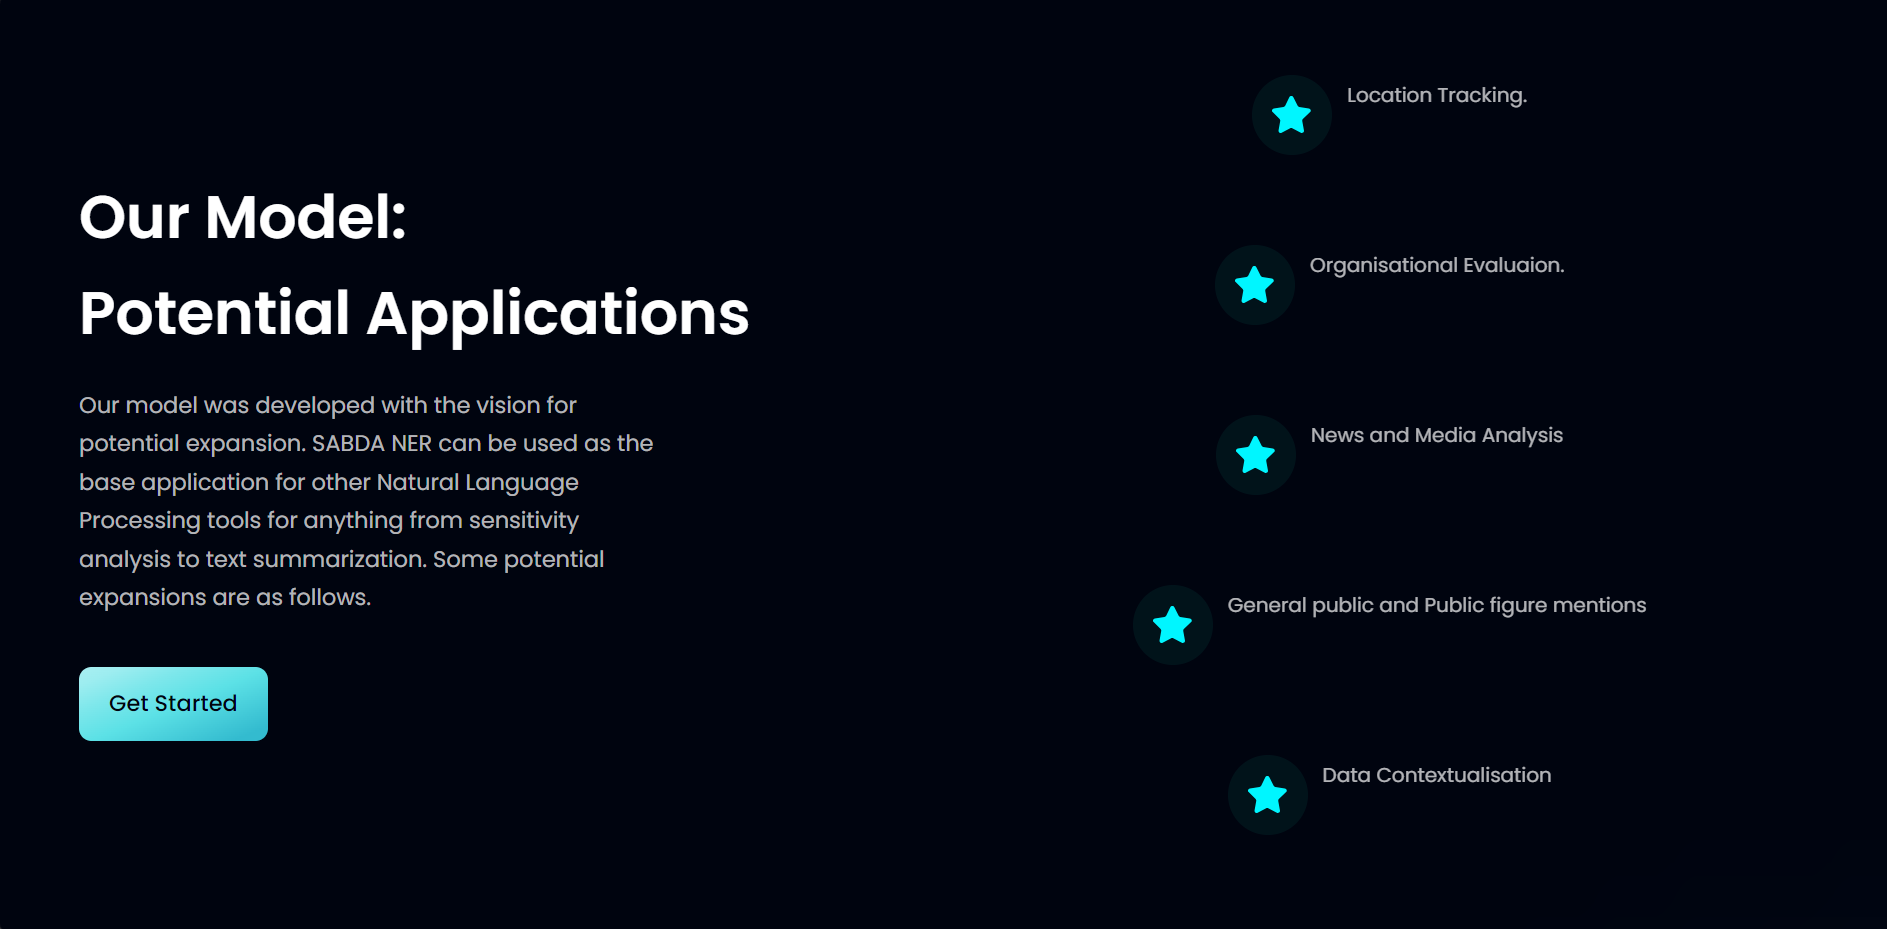
\includegraphics [scale=0.37]{img/UI/4applications.png}
 \caption[Potential Applications]{Potential Applications}
% \label{fig:DisplaCy.png}
\end{figure}

\vspace{30pt}

\begin{figure}[H]
\centering
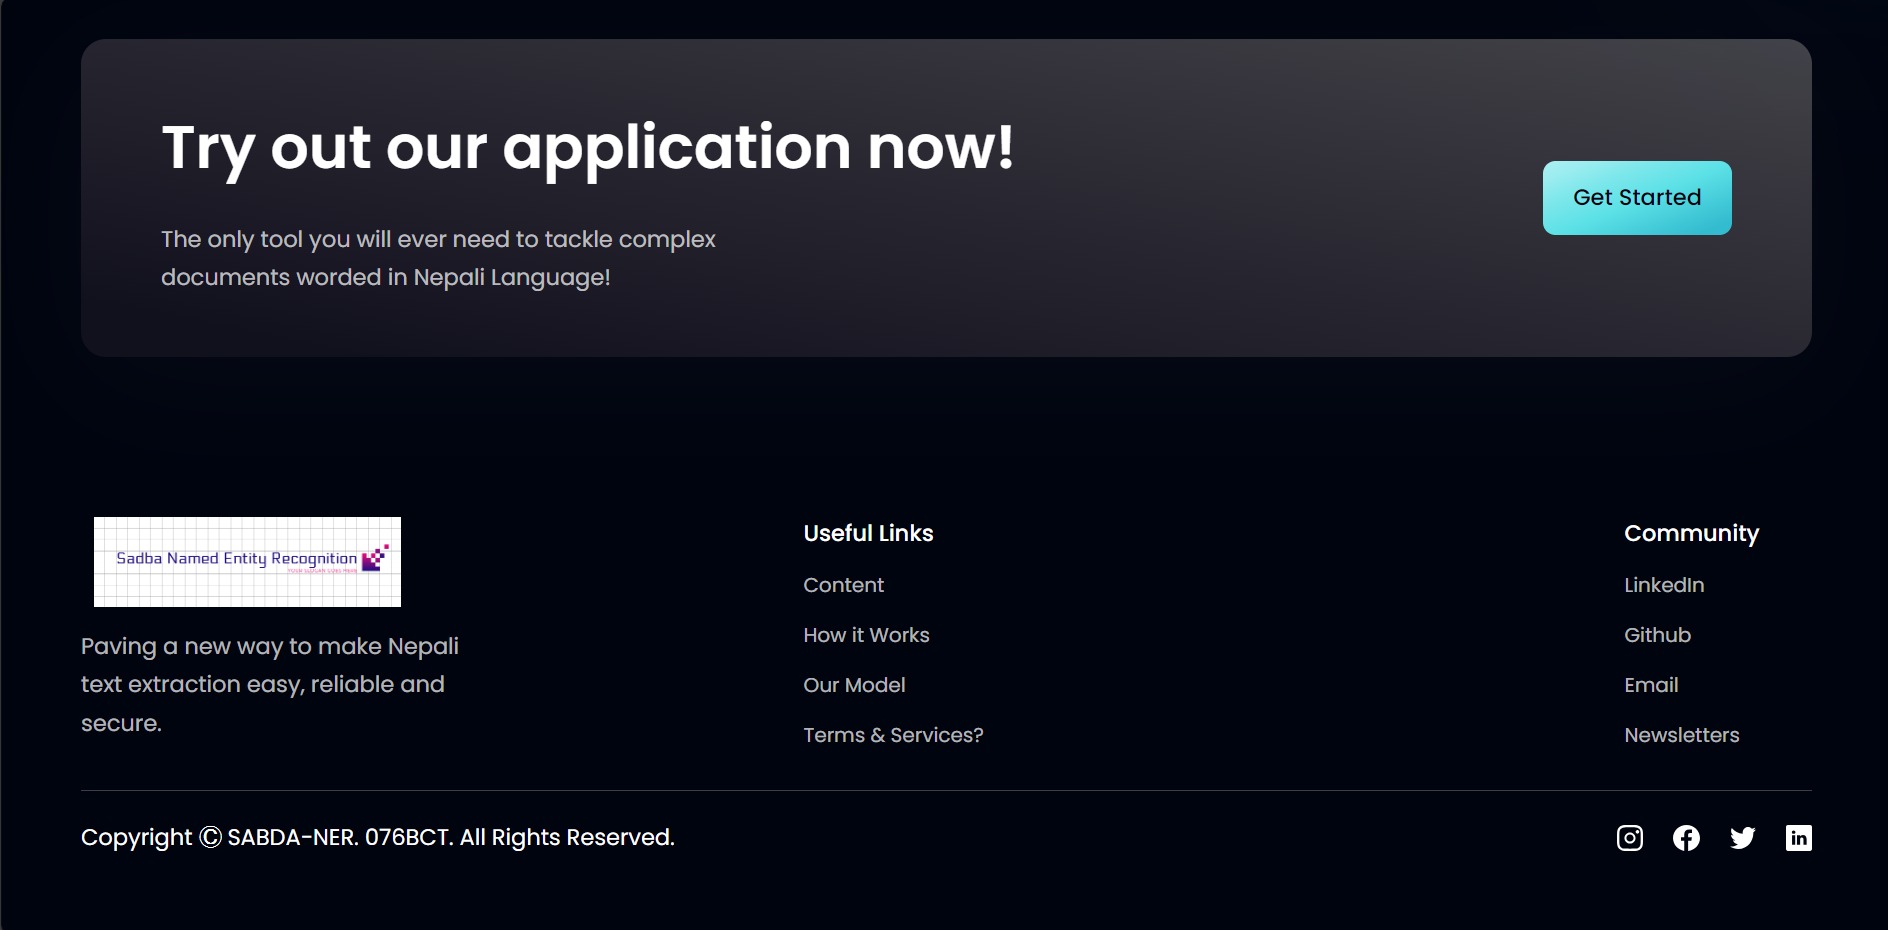
\includegraphics [scale=0.37]{img/UI/5footer.png}
 \caption[Footer Page]{Footer Page}
% \label{fig:DisplaCy.png}
\end{figure}